\documentclass[a4paper,titlepage]{article}

\usepackage[T1]{fontenc}
\usepackage[utf8]{inputenc}
\usepackage[italian]{babel}
\usepackage{listings}
\usepackage[dvips]{graphicx}
%\usepackage{syntonly}
%\syntaxonly

\pagestyle{headings}

%\includeonly{}

\lstset{
	language=C,
	frame=single,
	basicstyle=\footnotesize,
	tabsize=3,
	inputencoding=utf8,
	literate={==}{= =}{3}
}

\title{Reliable UDP}
\author{Simone Falvo}


\begin{document}

\maketitle

\begin{abstract}

Progetto e realizzazione di un'applicazione FTP distribuita di tipo client-server, utilizzando UDP come protocollo di trasporto.
L'applicazione implementa i classici comandi di un'applicazione FTP: LIST, GET e PUT, garantendo la possibilità di eseguire tali operazioni in parallelo per ogni client e l'integrità di messaggi e file scambiati.

\end{abstract}


\tableofcontents
\newpage

\section{Architettura}
Il sistema è composto da un server e molteplici client che scambiano dati in parallelo con il server, pertanto è necessario un server che sia in grado di gestire tutti i client contemporaneamente. Per prima cosa quindi, verrà descritto il modello di server scelto, poi verranno descritti i dettagli architetturali dettati dai requisiti funzionali.

\subsection{Scelta del modello}

La gestione contemporanea di più client viene realizzata da un server di tipo multi-processo.\\
La scelta di tale modello è stata effettuata tenendo conto dei seguenti criteri:
\begin{itemize}
\item Semplicità del codice
\item Tolleranza ai guasti
\item Efficienza
\item Utilizzo delle risorse di sistema
\end{itemize}
%La scelta è stata effettuata in base alle esigenze di un generico utente di un applicazione FTP.
Un'applicazione di questo tipo coinvolge file di grosse dimensioni, che vanno dalle centinaia di megabyte fino all'ordine dei gigabyte. Il trasferimento di tali file richiede tempi consideroveli dell'ordine dei minuti, per questo motivo è di fondamentale importanza che il trasferimento subisca meno intoppi possibili, in particolere è necessario che un fallimento riguardante la connessione con un client non coinvolga le altre connessioni. Si immagini, ad esempio, lo sconforto di un utente che dopo decine di minuti di download, si vede cadere la connessione a seguito di un problema sconosciuto e che non dipende da lui.\\
Questo fatto rende la gestione dei guasti il criterio dominante, pertanto si è scelto il modello di server a processi in cui le connessioni vengono gestite da singoli processi ``isolati'', nel senso che il fallimento di un processo non inficia in nessun modo l'esecuzione degli altri processi.

Se, con i processi, da un lato si ottiene tolleranza ai guasti, dall'altro si perde in efficienza, poiché si introduce un overhead significativo per la creazione dei processi ed il cambio di contesto.\\
Nonostante si sarebbe potuto ridurre l'overhead dovuto alla creazione dei processi tramite lo sviluppo di un modello a preforking, si è scelto di ignorare questa possibilità perché ciò avrebbe reso il codice più complesso a fronte di un miglioramento dei tempi di risposta trascurabile, infatti tali tempi sono dominati dal tempo di trasferimento del file che è di vari ordini di grandezza superiore a quello di generazione del processo.

\subsection{Stratificazione del sistema}
Per realizzare un'applicazione basata su UDP che garantisca una comunicazione 
affidabile è stato necessario introdurre a livello applicativo uno strato che
si ponesse logicamente tra applicazione e livello di trasporto e che astraesse
un protocollo di trasporto affidabile.\\
Tale strato di ``pseudo-trasporto'', (o livello di trasporto virtuale), fornisce un'interfaccia all'applicazione 
per mezzo delle funzioni \emph{rdt\_send} e \emph{rdt\_recv} simile a quella 
offerta dalle API \emph{sendto} e \emph{recvfrom} utilizzate per UDP, 
quindi tutto ciò che riguarda l'implementazione necessaria a garantire 
affidabilità è trasparente al livello applicativo puro.\\
Tuttavia la trasparenza non è del tutto completa perché, affinché questo strato
di trasporto virtuale funzioni, è necessario inizializzare le strutture che ne 
fanno parte, sia da un lato che dall'altro della comunicazione con gli stessi 
parametri. Questo implica che prima di poter comunicare in modo affidabile, 
client e server devono accordarsi sulla scelta dei parametri, in particolare, 
vengono impostati all'avvio del server, per poi essere inviati ai client che 
vogliono essere serviti.\\
Un'altra caratteristica utile, è che utilizzare la \emph{rdt\_recv}, è 
funzionalmente identico ad effettuare una \emph{read} da una socket in TCP, 
infatti è possibile effettuare letture successive dello stesso messaggio, senza 
che gli altri dati che si devono ancora leggere vadano persi. 


\section{Implementazione}
\subsection{Simulazione rete inaffidabile}
Il progetto è stato testato ed eseguito all'interno di una rete locale, pertanto è stato necessario simulare la perdita dei pacchetti.\\
Ciò è stato fatto introducendo delle opportune funzioni per l'invio dei dati, le quali inviano se e soltanto se viene estratto un numero casuale maggiore di una data probabilità di perdita.

\begin{lstlisting}[title=simul\_udt.c]
ssize_t udt_sendto(int sockfd, const void *buf, size_t len, 
				 const struct sockaddr *addr, socklen_t addrlen,
				 double loss)
{
	ssize_t retval = len;

	// necessary flow control into a local network
	if (loss < 0.1)
		usleep(50);

	if (randgen() > loss) 
		retval = sendto(sockfd, buf, len, 0, addr, addrlen);

	return retval;
}


ssize_t udt_send(int sockfd, void *buf, size_t size, double loss)
{
	return udt_sendto(sockfd, buf, size, NULL, 0, loss);
}


double randgen(void)
{
	static bool seed = false;
	if (!seed) {
		srand48(time(NULL));
		seed = true;
	}
	return drand48();
}
\end{lstlisting}

\subsection{Connessione}
La comunicazione tra client e server avviene a seguito dell'instaurazione di una connessione senza autenticazione.\\
Il client quando vuole connettersi al server invia un messaggio di SYN, dopodiché si mette in attesa di un messaggio di risposta (SYNACK) contenente i parametri necessari alfunzionamento del protocollo di communicazione affidabile. Questa attesa è limitata dalla presenza di un timer di 5 secondi, allo scadere del quale avviene un nuovo tentativo di connessione reinviando il messaggio di SYN.\\
Ricevuto il messaggio di risposta, vengono create ed inizializzate le strutture di comunicazione e la connessione risulta instaurata, da questo istante è possibile inviare comandi al server in modo affidabile.\\
Poiché, al momento della richiesta di connessione, non si dispone nemmeno del parametro relativo alla probabilità di perdita di un pacchetto, il messaggio di SYN viene inviato con probabilità di perdita pari al 20\%.

\begin{lstlisting}[title=client: instaurazione della connessione]
	...

/* set receiving timeout on the socket */
timeout.tv_sec = 5;
timeout.tv_usec = 0;
if (setsockopt
	(sockfd, SOL_SOCKET, SO_RCVTIMEO, &timeout, sizeof(timeout))
	== -1)
	handle_error("setting socket timeout");

while (!connected) {

	/* send SYN */
	if (udt_sendto(sockfd, NULL, 0, (struct sockaddr *) addr, 
		addrlen, 0.2) == -1)
		handle_error("udt_sendto() - sending SYN");
	fputs("SYN sent, waiting for SYN ACK\n", stderr);

	/* get SYN_ACK and server connection address */
	errno = 0;
	if (recvfrom
		(sockfd, &params, sizeof(params), 0,
		(struct sockaddr *) addr, &addrlen) == -1) {
		if (errno == EAGAIN || errno == EWOULDBLOCK)
			// timeout expired
			continue;
		handle_error("recvfrom()");
	}

	connected = true;
}

/* turn timeout off */
timeout.tv_sec = 0;
timeout.tv_usec = 0;
if (setsockopt
	(sockfd, SOL_SOCKET, SO_RCVTIMEO, &timeout, sizeof(timeout)) 
	== -1)
	handle_error("setting socket timeout");

/* set the endpoint */
if (connect(sockfd, (struct sockaddr *) addr, addrlen) == -1)
	handle_error("connect()");

/* initialize transport layer */
init_transport(sockfd, &params);

	...
\end{lstlisting}

I parametri necessari al protocollo di comunicazione affidabile  giungono
al client incapsulati in una struttura \emph{params} che contiene:
\begin{itemize}
\item[T]: intero senza segno a 16 bit che indica il timeout espresso in 
millisecondi;
\item[P]: intero senza segno a 8 bit che indica la probabilità di perdita di un
datagramma nella rete, espresso in percentuale (da 0 a 100);
\item[N]: intero senza segno a 8 bit che indica l'ampiezza della finestre di
invio e ricezione del protocollo selective repeat;
\item[adaptive]: intero senzo segno a 8 bit interpretato come valore booleano
che indica se il protocollo di comunicazione affidabile deve avere un timeout
di tipo adattativo per ogni segmento che viene inviato.
\end{itemize}

\begin{lstlisting}[title=basics.h]
struct proto_params {
	uint16_t T;
	uint8_t  P;
	uint8_t  N;
	uint8_t  adaptive;
};
\end{lstlisting}

Il server, costantemente in attesa di richieste di connessione, alla ricezione
di un messaggio di SYN, crea un processo figlio al quale affida il compito di 
inviare i parametri di connessione e di gestire la connessione con il client.

\begin{lstlisting}[title=server: instaurazione della connessione]

	...

for (;;) {

	clilen = sizeof(cliaddr);
	memset((void *) &cliaddr, 0, clilen);

	/* wait for connection requests */
	errno = 0;
	if (recvfrom
		(sockfd, buf, MAXLINE, 0, (struct sockaddr *) &cliaddr,
		 &clilen) == -1) {

		 if (errno == EINTR)
			// signal interruption
			continue;

		handle_error("waiting for connection requests");
	}

	/* create a new proccess to handle the client requests */
	pid = fork();

	if (pid == -1)
		handle_error("fork()");

	if (!pid) {                 // child process

		/* close duplicated listen socket */
		if (close(sockfd) == -1)
			handle_error("close()");

		create_connection(&params, &cliaddr, clilen);
	}
}

	......

\end{lstlisting}


Il processo figlio crea una nuova socket e tramite quest'ultima invia al client i parametri del protocollo di comunicazione affidabile.
Poi imposta l'indirizzo del client come destinazione prefissata, inizializza la connessione e rimane in attesa di eventuali comandi da parte del client.

\begin{lstlisting}[title=connessione del nuovo processo]
void create_connection(struct proto_params *params,
					   struct sockaddr_in *cliaddr, socklen_t clilen)
{
	int connsd;

	/* create a connection socket */
	if ((connsd = socket(AF_INET, SOCK_DGRAM, 0)) == -1)
		handle_error("socket()");

	/* set the end point */
	if (connect(connsd, (struct sockaddr *) cliaddr, clilen) == -1)
		handle_error("socket()");

	/* send SYN_ACK with protocol parameters */
	if (udt_send(connsd, params, sizeof(struct proto_params), 
		params->P / 100.0) == -1)
		handle_error("udt_send() - sending SYN_ACK");

	init_transport(connsd, params);

	server_job();
}
\end{lstlisting}


Un limite di questa implementazione consiste nel fatto che il server non sa distinguere se un SYN proviene da un nuovo client oppure è un tentativo di riconnessione, per cui, se si verifica il secondo caso, il processo server d'ascolto crea un nuovo figlio quando ce n'era già uno in attesa di richieste di quel client.
In questo modo se si perdono molteplici SYNACK destinati ad uno specifico client, verranno creati altrettanti processi server che rimarranno in attesa di richieste che non arriveranno mai.\\
Una possibile soluzione a questo problema sarebbe quella di far mantenere al server informazioni, di durata limitata, che permettano di capire se per il client che effettua la richiesta di connessione, esiste già un processo dedicato. In tal caso, basterebbe comunicare al processo figlio in questione di inviare di nuovo il messaggio di SYNACK.\\
Questa soluzione implicherebbe la gestione di una lista di associazioni client-pid, che andrebbe scandita ad ogni ricezione di messaggi SYN, e della comunicazione tra processo padre e processo figlio, quindi per motivi di efficenza e semplicità del codice, si è scelto di non implementarla.\\
Ad ogni modo un processo di connessione, se non riceve comandi per un tempo pari a 1 minuto, termina la propria esecuzione, liberando così preziose risorse.\\
(La gestione dei processi zombie verrà descritta più avanti).

\subsection{Protocollo di comunicazione}
In generale, il protocollo di comunicazione prevede che il client invii messaggi di comando in cui venga specificato il tipo di comando da eseguire, il server, quindi esegue il comando e invia un messaggio di risposta.\\
Ogni comando prevede un trasferimento file, quindi, a seconda del tipo di comando, o nel messaggio di comando o in quello di risposta viene allegato il file, con le informazioni necessarie alla sua corretta ricezione.\\
Ogni messaggio di comando e di risposta è composto da campi di un numero fissato di byte contenenti le informazioni necessarie all'interpretazione del messaggio.
Essendo un'applicazione distribuita, i campi vengono distinti utilizzando variabili la cui ampiezza (numero di bit) è indipendente dall'architettura della macchina, a tal proposito ogni campo informativo è composto dalle variabili definite in \emph{stdint.h}.\\ 
I primi 8 bit di un messaggio di comando indicano sempre il tipo di comando da eseguire e, a seconda del comando, possono avere o meno ulteriori informazioni.

\begin{lstlisting}[title=Costanti comandi]
// command codes
#define LIST 		0
#define GET 		1
#define PUT 		2

// response codes
#define GET_OK      0
#define GET_NOENT   1
#define PUT_SUCCESS 2
#define PUT_FAILURE 3
\end{lstlisting}


\renewcommand{\arraystretch}{1.5}
\begin{tabular}{|c|c|}
\hline
CMD &    ....    ....    ....    \\
\hline
\end{tabular}

\begin{tabular}{c}
8 bit 
\end{tabular}


Una volta impostati i vari campi in un buffer, se non va inviato un file, i dati vengono passati direttamente al livello di trasporto virtuale.\\
Se altrimenti, va inviato un file, viene chiamata la funzione \emph{send\_file}, i campi informativi vengono considerati un header per il file ed il tutto viene frammentato (per non allocare troppa RAM) e passato al livello sottostante.\\
Lato opposto il ricevente analizza uno alla volta i campi informativi, poi legge il file tramite la funzione \emph{recv\_file}.


\begin{lstlisting}[title=cmd\_commons.c]
void send_file(int fd, void *header, size_t file_size, 
				size_t header_size)								
{                                                                                                       
	int8_t buffer[MAX_BUFSIZE];                                                                         
	size_t buf_size, total_size;                                                                        
	unsigned int i, n;                                                                                  
																										
	total_size = header_size + file_size;                                                               
	n = total_size / MAX_BUFSIZE;                                                                       
																										
	memcpy(buffer, header, header_size);                                                                
																										
	for (i = 0; i <= n; i++) {                                                                          
																										
		// calculate last bytes to send                                         
		if (i == n) {           
			buf_size = total_size % MAX_BUFSIZE;                                                        
			if (!buf_size)                                                                              
				// total size is a multiple of MAX_BUFSIZE:
				// send only n-1 chunks        
				break;          
		} else                                                                                          
			buf_size = MAX_BUFSIZE;                                                                     
																										
		if (readn(fd, buffer + header_size, buf_size - header_size)
			== -1)                              
			handle_error("readn() - reading file to send");

		header_size = 0;  // consider header only at the first pass

		rdt_send(buffer, buf_size);
	}
}

void recv_file(int fd, size_t size)
{
	unsigned int i, n = size / MAX_BUFSIZE;
	size_t buf_size;
	int8_t buffer[MAX_BUFSIZE];
                                                                                              
	for (i = 0; i <= n; i++) {
                                                                                              
		// calculate last bytes to store 
		if (i == n) {           
			buf_size = size % MAX_BUFSIZE;
			if (!buf_size)
				// size is a multiple of MAX_BUFSIZE:
				// receive only n-1 chunks
				break;          
		} else
			buf_size = MAX_BUFSIZE;
                                                                                              
		rdt_recv(buffer, buf_size);
                                                                                              
		if (writen(fd, buffer, buf_size) == -1)
			handle_error("writen() - writing received file");
	}
}
\end{lstlisting}

\subsection{Trasferimento affidabile}
Il trasferimento affidabile è stato realizzato implementando l'algoritmo \emph{selective repeat} descritto nel libro [riferimento].\\
Tale implementazione è stata ``isolata'' all'interno di un modulo apposito, creando una sorta di livello di trasporto virtuale, il quale si occupa di suddividere i messaggi in segmenti di giusta misura e di gestirne gli invii, le ritrasmissionie la ricezione.

\subsubsection{Interfaccia}
L'interfaccia che offre questo stato di trasporto virtuale, come descritto nei primi capitoli, è simile a quella che un programmatore ha a disposizione per un protocollo TCP.\\
Per richiamare la funzione per l'invio dei dati (\emph{rdt\_send}) basta specificare l'indirizzo e la dimensione del buffer contente i dati da inviare, mentre per la ricezione (\emph{rdt\_recv}) l'indirizzo e la dimensione del buffer che riceverà i dati.\\
A differenza delle comuni \emph{read} e \emph{write} non va specificato il file descriptor della socket, perché il servizio di trasporto virtuale si basa su una connessione, per cui la socket è fissata al momento dell'instaurazione della connessione, che avviene quando viene chiamata la funzione \emph{init\_transport}.\\
Inoltre la funzione \emph{rdt\_read\_string} permette di leggere una stringa di una certa lunghezza massima dal messaggio arrivato, cosa necessaria per poter leggere il nome del file che si vuole scaricare.

\begin{lstlisting}[title=transport.h].
void init_transport(int sockfd, struct proto_params *params);
void rdt_send(const void *buf, size_t len);
void rdt_recv(void *buf, size_t len);
ssize_t rdt_read_string(char *buf, size_t size);
\end{lstlisting}

\subsubsection{Struttura}
Lo strato di trasporto virtuale è visto dall'esterno come una black box che 
prende in ingresso messaggi dal livello applicativo, e restituisce i messaggi
di risposta dell'host interlocutore.\\
Nello specifico un messaggio viene frammentato in segmenti di una misura 
massima prefissata (MSS), i quali poi vengono inviati e gestiti tramite 
l'algoritmo di trasferimento affidabile, in questo modo vi è la garanzia che 
un segmento non venga ulteriormente suddiviso a livello di collegamento.\\
La dimensione massima del segmento è stata calcolata considerando un MTU 
relativo ad un collegamento Ethernet standard di 1500 byte, un header UDP/IP
di 28 byte ed un header contente i parametri necessari all'esecuzione 
dell'algoritmo: il numero di sequenza del segmento pari ad 1 byte e la 
quantità di byte significativi nel payload pari a 2 byte.
Il numeri di sequenza sono contenuti in variaili da 8 bit, pertanto vanno 
da $0$ a MAXSEQNUM - 1, con MAXSEQNUM = $2^8$.

%MSS = MTU - UDP/IP - SR
\begin{lstlisting}[title=transport.h]

#define MAXSEQNUM       (1 << 8)
#define MTU             1500
#define UDPIP_HEADER    28
#define SR_HEADER       (sizeof(uint8_t) + sizeof(uint16_t))

#define MSS             (MTU - UDPIP_HEADER - SR_HEADER)


struct segment {
	uint8_t  seqnum;
	uint16_t size;
	uint8_t  payload[MSS];
};
\end{lstlisting}

Il livello di trasporto virtuale è composto principalmente da due servizi 
indipendenti:
\begin{itemize}
\item \textbf{send\_service}: servizio che si occupa dell'invio dei segmenti e
della gestione di gran parte del protocollo lato mittente.
\item \textbf{recv\_service}: servizio che si occupa principalmente della
ricezione di ack e segmenti, pertanto interpreta il lato destinatario del 
protocollo e collabora con il lato mittente.
\end{itemize}
Entrambi vengono implementati tramite thread, per renderli indipendenti dal 
thread principale ``applicativo'' e affinché sia possibile che un host invii 
segmenti e riceva ACK contemporaneamente.\\
L'operazione di creazione di questi thread, sia lato mittente che destinatario
(con gli stessi parametri), equivale all'instaurazione della connessione,
e viene eseguita dalla funzione \emph{init\_transport}.

\begin{lstlisting}[title=transport.c]
/* shared structures */
struct circular_buffer recv_cb;
struct circular_buffer send_cb;
struct event e;
/* threads args to keep alive */
struct shared_tools recv_tools, send_tools;


void init_transport(int sockfd, struct proto_params *params)
{
    pthread_t t;

    /* initialize circular buffers */

    recv_cb.E = recv_cb.S = 0;
    send_cb.E = send_cb.S = 0;

    /* initialize shared tools */

    recv_tools.sockfd = sockfd;
    recv_tools.e = &e;
    recv_tools.cb = &recv_cb;
    recv_tools.params = params;

    send_tools = recv_tools;
    send_tools.cb = &send_cb;

    /* initialize mutexes */

    if (pthread_mutex_init(&e.mtx, NULL) != 0)
        handle_error("pthread_mutex_init()");
    if (pthread_mutex_init(&recv_cb.mtx, NULL) != 0)
        handle_error("pthread_mutex_init()");
    if (pthread_mutex_init(&send_cb.mtx, NULL) != 0)
        handle_error("pthread_mutex_init()");

    /* initialize conditions */

    if (pthread_cond_init(&recv_cb.cnd_not_empty, NULL) != 0)
        handle_error("pthread_cond_init()");
    if (pthread_cond_init(&send_cb.cnd_not_empty, NULL) != 0)
        handle_error("pthread_cond_init()");

    if (pthread_cond_init(&recv_cb.cnd_not_full, NULL) != 0)
        handle_error("pthread_cond_init()");
    if (pthread_cond_init(&send_cb.cnd_not_full, NULL) != 0)
        handle_error("pthread_cond_init()");

    if (pthread_cond_init(&e.cnd_event, NULL) != 0)
        handle_error("pthread_cond_init()");
    if (pthread_cond_init(&e.cnd_no_event, NULL) != 0)
        handle_error("pthread_cond_init()");

    /* create threads */

    if (pthread_create(&t, NULL, recv_service, &recv_tools) != 0)
        handle_error("creating recv_service");

    if (pthread_create(&t, NULL, send_service, &send_tools) != 0)
        handle_error("creating send_service");
}
\end{lstlisting}

Il servizio di invio è stato implementato come un thread che rimane in attesa
fintanto che non avviene uno dei seguenti eventi:
\begin{itemize}
\item[-]Ricezione dati dal livello applicativo;
\item[-]Ricezione di un aknowledgment dalla rete;
\item[-]Scadenza di un timeout relativo ad un segmento inviato.
\end{itemize}

Il sistema di attesa è stato implementato tramite un meccanismo di segnalazione
di eventi basato su variabili di condizione.\\
Il thread infatti attende fintanto che non viene segnalata una condizione di
evento, dopodiché esso si sveglia ed in base al tipo di evento 
esegue il compito associato.\\
La struttura \emph{event} è composta dalle due variabili condizione 
\emph{cond\_event} e \emph{cond\_no\_event}, che indicano rispettivamento
il verificarsi di un evento ed il caso opposto, ovvero che non vi è un evento
da gestire, l'intero \emph{type} invece specifica il tipo di evento che si è
verificato e l'intero a 8 bit \emph{acknum} contiene il numero di sequenza del
segmento per il quale si è ricevuto un ack.

\begin{lstlisting}[title=event.h]
#define NO_EVENT	0
#define PKT_EVENT	1
#define ACK_EVENT	2

struct event {
	pthread_mutex_t mtx;
	pthread_cond_t cnd_event;
	pthread_cond_t cnd_no_event;
	unsigned int type;
	uint8_t acknum;
};

int cond_event_signal(struct event *e, unsigned int event_type);
int cond_ack_event_signal(struct event *e, uint8_t acknum);
\end{lstlisting}

La funzione \emph{cond\_event\_signal} permette di inviare un segnale che indica il
verificarsi della condizione \emph{cond\_event} relativa ad uno specifico tipo di 
evento.\\
La funzione \emph{cond\_ack\_event} è relativa soltanto all'avento di ricezione
di un ack, e permette, oltre che di segnalare l'evento, anche di specificare
il numero di sequenza del segmento per il quale si è ricevuto l'ack.

In questo modo vengono segnalati gli eventi di consegna di dati dall'applicazione
e di arrivo di un ack. La scadenza di un timeout invece avviene semplicemente 
impostando un tempo limite di attesa per la funzione \emph{pthread\_cond\_timedwait},
al termine del quale il thread si risveglia e verrà restituito il valore ETIMEDOUT 
che indica tale evento.

\begin{lstlisting}[title=transport.c]
void *send_service(void *p)
{
		.......

    if (pthread_mutex_lock(&e->mtx) != 0)
        handle_error("pthread_mutex_lock");

    for (;;) {

        e->type = NO_EVENT;
        if (pthread_cond_broadcast(&e->cnd_no_event) != 0)
            handle_error("pthread_cond_broadcast()");

        condret = 0;
        while (e->type == NO_EVENT && condret != ETIMEDOUT) {
            // no events and timeout not expired

		.......

            condret = pthread_cond_timedwait(&e->cnd_event,
                      &e->mtx, &wait_time);
            if (condret != 0 && condret != ETIMEDOUT)
                handle_error("pthread_cond_timedwait");
        }

        /* TIMEOUT EVENT */
        if (condret == ETIMEDOUT) {
            // timeout work .......
            continue;
        }

        switch (e->type) {

        case PKT_EVENT:
            // pkt work .......
            break;

        case ACK_EVENT:
            // ack work .......
            break;
        }
    }

    if (pthread_mutex_unlock(&e->mtx) != 0)
        handle_error("pthread_mutex_unlock");

		.......

}
\end{lstlisting}

L'accesso esclusivo alla variabile \emph{event} è garantito dalla presenza
del mutex come attributo della stessa.\\
Il thread di invio è acquisce il mutex appena viene instaurata la connessione
e lo rilascia soltanto tramite la \emph{pthread\_cond\_timedwait}, ovvero
quando si mette in attesa di un evento, pertanto non è possibile che la 
variabile venga acceduta durante la gestione di uno degli eventi.
Per quanto riguarda la concorrenza tra il thread principale e il thread di
ricezione, il primo che accede alla variabile tramite l'acquisizione del
mutex segnala il proprio evento, poi se il secondo accede e trova che il tipo
di evento è diverso da NO\_EVENT aspetta fintanto che il thread di invio 
non se ne occupa e segnala di nuovo l'assenza di eventi tramite la funzione
\emph{pthread\_cond\_broadcast}.

\begin{lstlisting}[title=event.c]
int cond_event_signal(struct event *e, unsigned int event_type)
{
    int retval = 0;

    if (pthread_mutex_lock(&e->mtx) != 0)
        retval = -1;

    else {

        // wait until no event is signaled
        while (e->type != NO_EVENT)
            if (pthread_cond_wait(&e->cnd_no_event, &e->mtx) != 0)
                retval = -1;

        e->type = event_type;

        if (pthread_cond_signal(&e->cnd_event) != 0)
            retval = -1;

        if (pthread_mutex_unlock(&e->mtx) != 0)
            retval = -1;
    }

    return retval;
}
\end{lstlisting}


Il servizio di ricezione invece risponde ai seguenti eventi:
\begin{itemize}
\item[-]Ricezione di dati dalla rete (segmenti o ack);
\item[-]Scadenza di un timeout relativo alla connessione.
\end{itemize}
In caso di ricezione di dati dalla rete, segmenti e ack vengono distinti in 
base alla loro dimensione, invece il timeout è implementato impostandolo
sulla socket in lettura.
\begin{lstlisting}[title=transport.c]
void *recv_service(void *p)
{
	.....

    for (;;) {

        r = read(sockfd, buffer, max_recvsize);

        if (r == -1) {
            if (errno == EINTR)
                // signal interruption
                continue;
            if (errno == EAGAIN || errno == EWOULDBLOCK) {
                // timeout expired: close connection
                puts("Connection expired\n");
                exit(EXIT_SUCCESS);
            }
            handle_error("recv_service - read()");
        }

        /* segment received */
        if (r == sizeof(struct segment)) {

            // segment work .....
            
            continue;
        }

        /* ACK received */
        if (r == sizeof(acknum)) {

            // ack work .....

            continue;
        }

        fputs("recv_service: undefined data received\n", stderr);
    }

	.....
}
\end{lstlisting}


Le funzioni \emph{rdt\_send} e \emph{rdt\_recv} fungono da regolatori del flusso
di dati dal livello applicativo puro a quello di trasporto virtuale e 
viceversa.\\
Queste funzioni comunicano con i thread di invio e ricezione tramite 
dei buffer condivisi secondo uno schema del tipo produttore-consumatore, in 
modo tale che i dati effettuino il passaggio di livello solo quando c'è spazio
disponibile sui buffer.

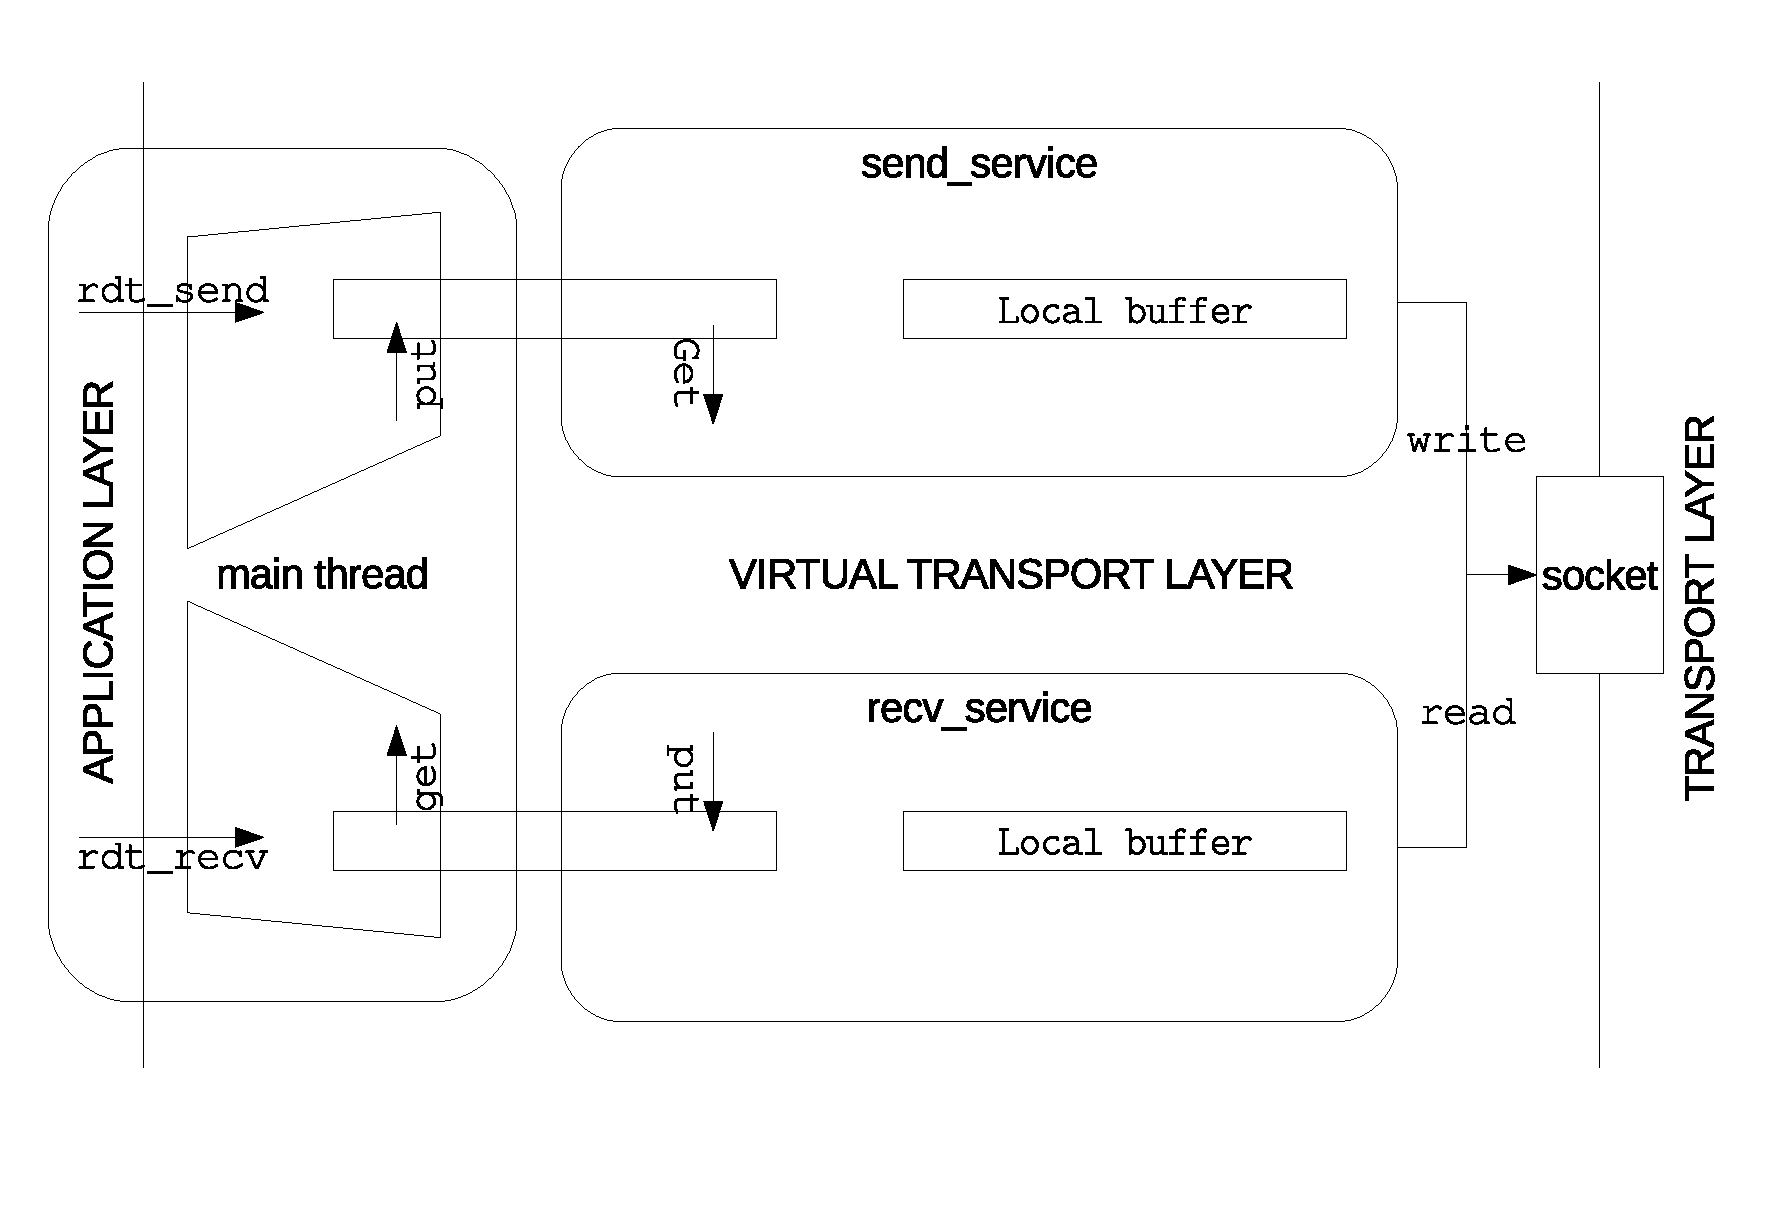
\includegraphics[scale=0.35]{images/structure_1}

Prima di passare a come viene implementato il \emph{selective repeat}, è 
necessario introdurre le strutture principale che ne supportano il 
funzionamento.\\
Come già detto, le unità di base con cui l'algoritmo ha a che fare sono
i segmenti che contengono i dati applicativi. Poiché tali segmenti sono
soggetti a ritrasmissioni, è necessario che vengano ``immagazzinati'' da 
qualche parte, inoltre, per quanto riguarda il lato destinatario, vanno
consegnati al livello applicativo in ordine, per queste ragioni, sia il 
servizio di invio che il servizio di ricezione sono dotati di buffer locali.\\
Tali buffer sono implementati tramite array di dimensione fissa e hanno una
capacità pari a MAXSEQNUM slot, in modo tale da far
corrispondere gli indici ai numeri di sequenza dei segmenti e 
garantirne un accesso immediato ($\mathcal{O}(1)$). Inoltre i buffer vengono
trattati come circolari, così da emulare naturalmente il riciclo dei numeri 
di sequenza.\\
Mentre il buffer del \emph{recv\_service} è implementato tramite un'array di 
strutture \emph{segment}, quello del \emph{send\_service} è un'array di 
strutture \emph{packet}, ovvero contenitori di segmenti e informazioni ad essi
relative necessarie al funzionamento del timeout, come istante di invio, quello
di scadenza ed un booleano che indica se il pacchetto è stato ritrasmesso.

\begin{lstlisting}[title=transport.h]
struct packet {
	struct segment sgt;
	struct timespec sendtime;
	struct timespec exptime;
	bool rtx;
};
\end{lstlisting}

Un'altra struttura fondamentale per l'algoritmo è la \emph{window}, che 
rappresenta le finestre di spedizione o ricezione delle due parti 
coinvolte.
\begin{lstlisting}[title=window.h]
struct window {
	unsigned int base;
	unsigned int width;
	struct bit_array ack_bar;	// 128 bit array
};
\end{lstlisting}
Tale struttura è composta da un'indice \emph{base} che rappresenta la base
della finestra, un intero \emph{width} che indica l'ampiezza massima della
finestra ed infine una struttura \emph{bit\_array} che non è altro che una
bitmask che tiene conto di quali segmenti sono arrivati a destinazione a 
partire dalla base della finestra.

[Disegno esempio bitmask] 

Infine, vi è la struttura necessaria alla gestione del timeout dei segmenti
inviati: una coda priotritaria i cui nodi sono puntatori
ai pacchetti presenti nel buffer locale di invio.\\
Ogni nodo è ordinato in base alla scadenza del timeout e una scansione 
periodica determina quali segmenti vanno ritrasmessi, appena si trova un 
segmento non scaduto non è necessario controllare i successivi
nella coda.
Questo meccanismo permette di gestire più timeot logici avendo un solo 
contatore hardware a disposizione.\\
In termini di prestazioni, avendo già N nodi nella coda, 
l'inserimento di un nuovo nodo richiede il confronto con tutti i
nodi che scadono prima, questo si effettua al più con un numero di passi
pari al numero di nodi presenti ($\mathcal{O}(N)$)
nel caso di timeout adattativo, invece se il timeout è costante non vi è bisogno
di alcun confronto poiché l'ultimo nodo inviato sarà l'ultimo a scadere e 
verrà semplicemente accodato (tempo $\mathcal{O}(1)$).
Per quanto riguarda l'estrazione del primo nodo da ritrasmettere, grazie 
all'inserimento prioritario, non è richiesta nessuna scansione, poiché il nodo 
in testa sarà il primo a scadere.\\
La coda è stata implementata in maniera tale da occupare meno memoria possibile,
infatti i nodi sono composti dagli indirizzi delle strutture \emph{packet}
presenti nel buffer locale, la coda tiene conto solo del loro ordinamento.

[disegno time\_queue]



\subsection{Trasferimento affidabile: selective repeat}
%
Il trasferimento affidabile è stato realizzato implementando l'algoritmo 
\emph{selective repeat} descritto in \cite{kurose}.
%
\subsubsection{Mittente}
%
Il lato mittente del protocollo viene svolto principalmente dal 
\emph{send\_service} e in parte anche dal \emph{recv\_service}.\\
Quando il lato applicativo intende inviare un messaggio, richiama la funzione
\emph{rdt\_send} passando dati e relativa quantità in byte come argomenti.\\
La funzione controlla lo spazio disponibile sul buffer circolare condiviso
e immette un quantità di dati (in byte) possibilmente pari ad un multiplo di 
MSS, per consentire al servizio di invio di creare segmenti completamente pieni 
di dati significativi (size = MSS). Se non sono disponibili almeno MSS byte 
aspetta fintanto che non si libera lo spazio necessario. Naturalmente il 
processo viene ripetuto fintanto che non vengono passati tutti i dati 
applicativi.\\
Essendo, il buffer circolare, una risorsa condivisa tra thread principale e 
thread di invio, è stato necessario implementare dei meccanismi di 
sincronizzazione.\\
A tale scopo l'accesso esclusivo al buffer viene garantito da un mutex,
mentre, per quanto riguarda l'attesa per la disponibilità di spazio, il thread
principale attende su una variabile condizione che viene opportunamente segnalata
quando il servizio di invio svuota il buffer. A sua volta il thread principale
segnala la condizione al thread di invio che nel buffer sono presenti dati dopo
l'immissione degli stessi.
%
\begin{lstlisting}[title=trasport.h]
struct circular_buffer {
    pthread_mutex_t mtx;
    pthread_cond_t cnd_not_empty;
    pthread_cond_t cnd_not_full;
    unsigned int S;
    unsigned int E;
    char buf[CBUF_SIZE];
};
\end{lstlisting}
\begin{lstlisting}[title=trasport.c]
void rdt_send(const void *buf, size_t len)
{
    size_t free, tosend, left = len;

    while (left) {

        if (pthread_mutex_lock(&send_cb.mtx) != 0)
            handle_error("pthread_mutex_lock");

        /* check available space */
        while ((free =
                space_available(send_cb.S, send_cb.E, CBUF_SIZE))
				<= MSS)
            if (pthread_cond_wait(&send_cb.cnd_not_full, 
				&send_cb.mtx) != 0)
                handle_error("pthread_cond_wait");

        /* calculate how much data to send */
        tosend =  free > left ?	left : free / MSS * MSS;

        memcpy_tocb(send_cb.buf, buf + len - left, tosend, 
					send_cb.E, CBUF_SIZE);

        send_cb.E = (send_cb.E + tosend) % CBUF_SIZE;

        if (pthread_mutex_unlock(&send_cb.mtx) != 0)
            handle_error("pthread_mutex_unlock");

        if (cond_event_signal(&e, PKT_EVENT) == -1)
            handle_error("cond_event_signal()");

        left -= tosend;
    }
}
\end{lstlisting}
%
Segnalata la presenza di dati sul buffer condiviso, il servizio di invio,
appena può, richiama la funzioni \emph{empty\_buffer} e \emph{send\_packets}.
%
\begin{lstlisting}[title=transport.c]
	.....

switch (e->type) {

case PKT_EVENT:

	/* empty shared buffer and put segments into the local one */
	empty_buffer(cb, pkts_buffer, &w, &lastseqnum);
	/* send available segments */
	send_packets(sockfd, loss, pkts_buffer, lastseqnum, &w,
				 &time_queue, &timeout);

	break;

case ACK_EVENT:
    // ack work .....
	break;

default:
	fputs("Unexpected event type\n", stderr);
	break;
}
	.....

\end{lstlisting}
%
La funzione \emph{empty\_buffer} ha il compito di svuotare il buffer condiviso,
creare i segmenti ed immagazzinarli nel buffer locale, in cui vi rimarranno
(saranno validi) fino a quando non sarà tornato indietro l'ack relativo e 
tutti quelli dei segmenti con numero di sequenza precedente.
%
\begin{lstlisting}[title=transport.c]
void empty_buffer(struct circular_buffer *cb, struct packet *pkts,
                  struct window *w, unsigned int *last_seqnum)
{
    size_t data, size;

    if (pthread_mutex_lock(&cb->mtx) != 0)
        handle_error("pthread_mutex_lock");

    while (cb->S != cb->E && 
           cbuf_free(w->base, *last_seqnum, MAXSEQNUM)) {
        // shared buffer not empty and local buffer has free slots

        data = data_available(cb->S, cb->E, CBUF_SIZE);
        size = data < MSS ? data : MSS;

        /* store a new packet */
        store_pkt(pkts, *last_seqnum, size, cb);
        *last_seqnum = (*last_seqnum + 1) % MAXSEQNUM;
        cb->S = (cb->S + size) % CBUF_SIZE;

        if (pthread_cond_signal(&cb->cnd_not_full) != 0)
            handle_error("pthread_cond_signal");
    }

    if (pthread_mutex_unlock(&cb->mtx) != 0)
        handle_error("pthread_mutex_unlock");
}
\end{lstlisting}
%
La funzione, fintanto che sono presenti dati sul buffer condiviso e ci sono 
slot liberi in quello locale, estrae al più MSS byte per poi creare un segmento,
che verrà posizionato in uno slot del buffer locale tramite la 
funzione \emph{store\_pkt}.\\
Ogni volta che un segmento viene estratto ed inserito nel buffer locale, viene anche 
aggiornato l'indice \emph{last\_seqnum} che indica il numero di sequenza del
prossimo pacchetto che verrà immagazzinato e quindi corrisponde al primo slot
libero del buffer locale.
%
\begin{lstlisting}[title=transport.c]
void store_pkt(struct packet *base, uint8_t seqnum, size_t size,
               struct circular_buffer *cb)
{
    struct packet *pkt = base + seqnum;
    struct segment *sgt = &(pkt->sgt);

    sgt->seqnum = seqnum;
    sgt->size = size;
    memcpy_fromcb(sgt->payload, cb->buf, size, cb->S, CBUF_SIZE);

    pkt->rtx = false;
}
\end{lstlisting}
%
La funzione \emph{send\_packets} si occupa di inviare i segmenti presenti nel
buffer locale fino a che l'indice nextseqnum non supera il limite stabilito
dall'ampiezza della finestra di invio.
%
\begin{lstlisting}[title=transport.c]
void send_packets(int sockfd, double loss, struct packet *pkts,
                  unsigned int lastseqnum, struct window *w,
                  struct queue_t *time_queue, 
				  struct timespec *timeout)
{
    static unsigned int nextseqnum = 0;
    struct packet *pkt;         // packet pointer

    while (in_window(w, nextseqnum) &&
           more_packets(nextseqnum, w->base, lastseqnum)) {
        // nextseqnum is inside the window and
        // there are packets not sent yet

        pkt = pkts + nextseqnum;
        send_packet(sockfd, pkt, loss);

        /* set packet sendtime and exptime */
        pkt_settime(pkt, timeout);

        prio_enqueue(pkt, time_queue, pkt_exptimecmp);
        nextseqnum = (nextseqnum + 1) % MAXSEQNUM;
    }
}
\end{lstlisting}
%
Quando un segmento viene inviato vengono registrati il tempo di invio e di
scadenza, inoltre un riferimento al pacchetto viene inserito nella coda 
per la gestione del timeout.\\
Una volta che almeno un segmento è stato inviato, entra in gioco il 
\emph{recv\_service} che, bloccato in lettura sulla socket, attende l'arrivo
degli ack.
Quando ne giunge uno, appena possibile, lo segnala al \emph{send\_service} 
inserendo il numero di sequenza nella variabile \emph{acknum} della
struttura condivisa \emph{event}.
%
\begin{lstlisting}[title=transport.c]
.....

for (;;) {

	r = read(sockfd, buffer, max_recvsize);

	.....

	/* segment received */
	if (r == sizeof(struct segment)) {
		// segment work .....
		continue;
	}

	/* ACK received */
	if (r == sizeof(acknum)) {
		acknum = (uint8_t) * buffer;
		if (cond_ack_event_signal(e, acknum) == -1)
			handle_error("cond_event_signal()");
		continue;
	}

.....
\end{lstlisting}
%
Alla ricezione del segnale di ack il servizio di invio rimuove il nodo 
corrispondente al numero di sequenza dell'ack, aggiorna il valore 
del timeout e aggiorna la finestra, eventualmente facendola scorrere 
se il numero di sequenza è relativo alla base della finestra.
%
\begin{lstlisting}[title=transport.c]
switch (e->type) {

    case PKT_EVENT:
        // pkt work .....
        break;

    case ACK_EVENT:
        acknum = e->acknum;
        if (params->adaptive)
            update_timeout(&timeout, pkts_buffer + acknum);
		remove_pkt_timeout(&time_queue, acknum);
        update_window(&w, acknum);
        empty_buffer(cb, pkts_buffer, &w, &lastseqnum);
        send_packets(sockfd, loss, pkts_buffer, lastseqnum, &w,
                     &time_queue, &timeout);
        break;

    default:
        fputs("Unexpected event type\n", stderr);
        break;
    }
}
\end{lstlisting}
Il valore del timeout viene aggiornato soltanto quando arrivano ack relativi
a segmenti che non hanno subito ritrasmissioni.\\
La funzione \emph{adapt\_timeout} aggiorna il timeout in base a quanto tempo
è trascorso dall'invio del segmento fino alla ricezione dell'ack, come
descritto nel libro di testo \cite{kurose}, secondo la formula [formula].
%
%	FORMULA
%
Il tempo trascorso è calcolato sottraendo all'istante corrente quello di invio
del segmento ricevuto, questo risulterà leggermente maggiore, perché
non viene calcolato nel momento esatto in cui arriva effettivamente l'ack.
%
\begin{lstlisting}[title=transport.c]
void update_timeout(struct timespec *timeout, struct packet *pkt)
{
    struct timespec now, elapsed;

    /* check if packet was retransmitted */
    if (pkt->rtx)
        return;

    if (clock_gettime(CLOCK_REALTIME, &now) == -1)
        handle_error("ack timestamp");

    if (timespec_sub(&elapsed, &now, &pkt->sendtime) == -1)
        handle_error("calculating elapsed time");

    adapt_timeout(timeout, &elapsed);
}
\end{lstlisting}
L'aggiornamento della finestra consiste nel contrassegnare il segmento come
ricevuto. Questo viene fatto impostando il relativo bit a 1 nella barra degli
ack della finestra.\\
Se il numero di sequenza corrisponde alla base della finestra, il bit non viene
impostato e viene fatta scorrere la finestra relativamente al prossimo segmento
per cui deve ancora arrivare un riscontro.
\begin{lstlisting}[title=window.c]
void update_window(struct window *w, uint8_t acknum)
{
    unsigned int i, s;

    if (acknum == w->base) {
        /* shift ack bar to the first unmarked bit */
        s = calc_shift(w);
        if (shift(&w->ack_bar, s) == -1)
            handle_error("shift()");
        /* slide window */
        w->base = (w->base + s) % MAXSEQNUM;
    }
    else if (in_window(w, acknum)) {
        /* calculate distance from window's base */
        i = distance(w, acknum);
        /* mark packet as acked */
        if (set_bit(&w->ack_bar, i) == -1)
            handle_error("set_bit()");
    }
}
\end{lstlisting}
Infine, se c'è stato uno scorrimento della finestra di invio, si libererà
dello spazio sul buffer circolare e sarà possibile 
inviare i segmenti successivi, pertanto vengono richiamate le funzioni
\emph{empty\_buffer} e \emph{send\_packets} già descritte in precedenza.\\
%
L'ultimo evento a cui il mittente deve reagire riguarda la scadenza del 
timeout di un segmento.\\
Ciò avviene quando la \emph{pthread\_cond\_timedwait} restituisce la 
costante ETIMEDOUT come valore di ritorno, in tal caso viene chiamata
la funzione \emph{resend\_expired} che determina quali pacchetti sono 
scaduti e li ritrasmette.
\begin{lstlisting}[title=window.c]
for (;;) {

    .....

	condret = 0;
	while (e->type == NO_EVENT && condret != ETIMEDOUT) {
		// no events and timeout not expired

		/* calculate remaining time to wait */
		if (calc_wait_time(&time_queue, &wait_time) == -1) {
			/* timeout expired: resend expired packets */
			resend_expired(sockfd, loss, &time_queue, &timeout, &w);
			continue;
		}

		condret = pthread_cond_timedwait(&e->cnd_event, &e->mtx,
                                         &wait_time);
		if (condret != 0 && condret != ETIMEDOUT)
			handle_error("pthread_cond_timedwait");
	}


	/* TIMEOUT EVENT */
	if (condret == ETIMEDOUT) {
		resend_expired(sockfd, loss, &time_queue, &timeout, &w);
		continue;
	}

    .....
}
\end{lstlisting}
La funzione per la ritrasmissione estrae segmenti fintanto
che non ne trova uno che non sia scaduto, ognuno di essi viene ritrasmesso,
marcato come tale, e vengono aggiornati i tempi di invio e di
scadenza, infine viene di reinserito nella coda del timeout.
\begin{lstlisting}[title=transport.c]
void resend_expired(int sockfd, double loss, 
                    struct queue_t *time_queue,
                    struct timespec *timeout, struct window *w)
{
    struct packet *pkt;

    while (time_queue->head != NULL) {

        /* fetch first to expire packet */
        pkt = get_head_packet(time_queue);

        if (!pkt_expired(pkt))
            break;

        dequeue(time_queue);

        send_packet(sockfd, pkt, loss);
        pkt->rtx = true;

        /* set packet time */
        pkt_settime(pkt, timeout);

        prio_enqueue(pkt, time_queue, pkt_exptimecmp);
    }
}
\end{lstlisting}
La funzione \emph{pthread\_cond\_timedwait} attende il verificarsi degli 
eventi di ricezione di dati dal livello superiore, oppure di ricezione di
un ack, per un tempo calcolato ad ogni ciclo tramite la funzione
\emph{calc\_wait\_time}, che imposta il tempo di attesa in base a quanto 
ne rimane alla scadenza del timeout del primo segmento.\\
Se la coda non contiene nodi, il timeout viene impostato ad un valore
abbastanza elevato per fare in modo che il thread non venga svegliato 
inutilmente, è sufficiente impostarlo nell'ordine delle decine di secondi.
\begin{lstlisting}[title=transport.c]
int calc_wait_time(struct queue_t *q, struct timespec *wait_time)
{
    struct packet *pkt;
    struct timespec now, left;

    if (clock_gettime(CLOCK_REALTIME, &now) == -1)
        handle_error("clock_gettime()");

    if (!q->head) {
        /* queue is empty: turn off the timeout */
        left.tv_sec = 30;
        left.tv_nsec = 0;
    } else {
        pkt = get_head_packet(q);

        /* calculate remaining time to timeout */
        if (timespec_sub(&left, &pkt->exptime, &now) == -1)
            /* now > exptime: timeout expired */
            return -1;
    }

    timespec_add(wait_time, &now, &left);
    return 0;
}
\end{lstlisting}

\subsubsection{Selective Repeat: ricevente}
Il lato mittente del protocollo viene svolto soltanto dal 
\emph{recv\_service}, che si occupa di gestire il riordino
e la consegna a livello applicativo dei segmenti che giungono 
dalla rete, ed eventualmente di inviare i riscontri al mittente.
\begin{lstlisting}[title=transport.c]
void *recv_service(void *p)
{
    .....

    for (;;) {

        r = read(sockfd, buffer, max_recvsize);

        if (r == -1) {
            // error ot timeout .....     
        }

        /* segment received */
        if (r == sizeof(struct segment)) {

            sgt = (struct segment *) buffer;
            if (process_segment(
                sgt, segments_cb, &recv_window, cb)) {
                /* send ACK */
                if (udt_send
                    (tools->sockfd, &sgt->seqnum, sizeof(uint8_t),
                     loss) == -1)
                    handle_error("udt_send() - sending ACK");
            }
            continue;
        }

        /* ACK received */
        if (r == sizeof(acknum)) {
            // ACK work .....
            continue;
        }
    }
    .....
}
\end{lstlisting}
Il thread, bloccato in lettura sulla socket, quando riceve un segmento
chiama la funzione \emph{process\_segment} che controlla il numero di 
sequenza. Se questo cade all'interno della finestra, si controlla se non
è un duplicato ed in tal caso il segmento viene salvato nel buffer locale
e viene marcato come ``giunto'' impostando ad 1 il bit relativo nella finestra,
poi, se coincide con la base della finestra, vengono consegnati a livello 
applicativo tutti i segmenti
consecutivi presenti nel buffer a partire dalla base, infine la funzione
restituisce \emph{true} per segnalare che il segmento è valido ed 
è necessario inviare l'ack al mittente.\\
Se il numero di sequenza cade nell'intervallo precedente alla base della
finestra \emph{[base - ampiezza; base - 1]},
il segmento è già stato ricevuto e quindi 
viene ignorato, ma la funzione restituisce comunque il valore \emph{true}
poiché è necessario inviare l'ack.\\
In tutti gli altri casi, un eventuale segmento viene ignorato e la funzione 
restituisce false per non far inviare il relativo ack al mittente.
\begin{lstlisting}[title=transport.c]
bool process_segment(struct segment *sgt, 
                     struct segment *segments_cb,
                     struct window *w, struct circular_buffer *cb)
{
    static unsigned int S = 0;
    unsigned int i, s, seqnum;

    seqnum = sgt->seqnum;
    fprintf(stderr, "received segment %u\n", seqnum);

    if (in_window(w, seqnum)) {

        /* calculate seqnum distance from the base of the window */
        i = distance(w, seqnum);

        /* check if the segment is a duplicate */
        if (is_duplicate(w, i)) {
            //fputs("Already received\n", stderr);
            return true;
        }

        /* store the segment */
        segments_cb[(S + i) % w->width] = *sgt;

        /* mark segment as arrived */
        if (set_bit(&w->ack_bar, i) == -1)
            handle_error("set_bit()");
        fprint_window(stderr, w);

        if (seqnum == w->base) {
            /* calculate the number of consecutive segments */
            s = calc_shift(w);
            /* deliver consecutive segments */
            for (i = 0; i < s; i++) {
                deliver_segment(cb, segments_cb + S);
                S = (S + 1) % w->width;
            }
            /* update window indexes */
            shift_window(w, s);
            w->base = (w->base + s) % MAXSEQNUM;
        }
        return true;
    } else if (in_prewindow(w, seqnum)) {
        //fputs("Already received\n", stderr);
        return true;
    }
    return false;
}
\end{lstlisting}
Nel caso in cui il numero di sequenza coincide con la base della finestra,
vengono contati i bit consecutivi impostati ad 1 e, successivamente, 
vengono consegnati a livello applicativo altrettanti segmenti (a partire 
da quello appena arrivato) tramite la funzione \emph{deliver\_segment}, 
che ne immette il payload nel buffer circolare condiviso appena c'è spazio
disponibile.
\begin{lstlisting}[title=transport.c]
void deliver_segment(struct circular_buffer *cb, 
                     struct segment *sgt)
{
    if (pthread_mutex_lock(&cb->mtx) != 0)
        handle_error("pthread_mutex_lock");

    /* check free space */
    while (space_available(cb->S, cb->E, CBUF_SIZE) <= MSS) 
        if (pthread_cond_wait(&cb->cnd_not_full, &cb->mtx) != 0)
            handle_error("pthread_cond_wait");

    memcpy_tocb(cb->buf, sgt->payload, sgt->size, cb->E, 
                CBUF_SIZE);
    cb->E = (cb->E + sgt->size) % CBUF_SIZE;

    if (pthread_cond_signal(&cb->cnd_not_empty) != 0)
        handle_error("pthread_cond_signal");
    if (pthread_mutex_unlock(&cb->mtx) != 0)
        handle_error("pthread_mutex_unlock");
}
\end{lstlisting}


\subsection{Gestione dei processi}
Una questione non trascurabile è sicuramente quella legata alla gestione
dei processi del sistema.\\
Essendo il server un modello multiprocesso, è fondamentale che ci sia un 
giusto controllo sui processi, in particolare è necassario che ogni 
processo termini la propria esecuzione se il client di cui si occupa non
effettua richieste.\\
Affinché ciò si verifichi, il servizio di ricezione rimane bloccato in 
lettura sulla socket per un tempo limitato, infatti se non riceve segmenti
in questo arco di tempo, viene chiamata la \emph{exit()} ed il processo 
termina. In tal caso la connessione viene considerata scaduta.
\begin{lstlisting}[title=transport.c]
void *recv_service()
{
    .....

    /* set connection timeout */
    timeout.tv_sec = 60;
    timeout.tv_usec = 0;
    if (setsockopt(sockfd, SOL_SOCKET, SO_RCVTIMEO, &timeout, 
        sizeof(timeout)) == -1)
        handle_error("recv_service - setting socket timeout");

    for (;;) {

        r = read(sockfd, buffer, max_recvsize);
        if (r == -1) {
            if (errno == EINTR)
                // signal interruption
                continue;
            if (errno == EAGAIN || errno == EWOULDBLOCK) {
                // timeout expired: close connection
                puts("Connection expired");
                exit(EXIT_SUCCESS);
            }
            handle_error("recv_service - read()");
        }

        /* segment received */
        .....

        /* ACK received */
        .....
    }
    .....
}
\end{lstlisting}
Quando un processo server termina la propria esecuzione, invia il segnale
SIGCHILD al processo server principale, che viene subito intercettato in 
modo tale che possano essere liberate le risorse.\\
Prima della creazione dei processi figli, il processo padre effettua la
la registrazione di un handler per il segnale SIGCHILD, il quale 
chiama la funzione  \emph{wait\_pid} in maniera non bloccante soltanto quando 
se ne ha effettivamente bisogno.
\begin{lstlisting}[title=server.c]
int main()
{
    ..... 

    /* bind the socket to the address */
    if (bind(sockfd, (struct sockaddr *) &servaddr, 
             sizeof(servaddr)) == -1)
        handle_error("bind()");

    /* register SIGCHLD signal handler */
    register_zombie_handler();

    for (;;) {
        /* wait for connection requests */
        /* create a new proccess to handle the client requests */
        ..... 
    }
    .....
}

void register_zombie_handler(void)
{
    struct sigaction sa;

    sa.sa_handler = sig_zombie_handler;
    sa.sa_flags = SA_RESTART;
    sigemptyset(&sa.sa_mask);

    if (sigaction(SIGCHLD, &sa, NULL) == -1)
        handle_error("sigaction()");
}

void sig_zombie_handler(int sig)
{
    pid_t pid;
    (void) sig;

    while ((pid = waitpid(-1, NULL, WNOHANG)) > 0)
        ;

    return;
}
\end{lstlisting}


\section{Analisi delle prestazioni}
\subsection{Ambiente di sviluppo}
Il sistema è stato sviluppato e testato su una macchina con le seguenti
caratteristiche:
\begin{itemize}
\item \textbf{SO}: Fedora 25, 64 bit, Linux kernel 4.13
\item \textbf{Processore}: 4 x Intel core i7-2620M CPU @ 2.70GHz
\item \textbf{RAM}: 3.8 GiB 
\end{itemize}
Tecnologie utilizzate:
\begin{itemize}
\item \textbf{Editor}: Vim 
\item \textbf{Compilatore}: GCC 6.4.1 
\end{itemize}

\subsection{Prestazioni}
Il sistema è stato analizzato eseguendo client e server sulla stessa 
macchina, sfruttando l'interfaccia di loopback.\\
Le prestazioni sono state analizzate facendo variare i paramatri T, P e N
uno alla volta.\\
Per effettuare un'analisi automatica e soddisfacente delle prestazioni 
sono stati opportunamente modificati i moduli \emph{server.c} e 
\emph{client.c}.\\
Il server è stato modificato in modo che facesse variare il parametro
desiderato ad ogni richiesta di un client. In altre parole si ottiene
un insieme di processi che gestiscono ognuno una connessione con un valore
del parametro diverso.
\begin{lstlisting}[title=server\_test.c]
    .....

for (params.N = MIN_WIDTH; params.N <= MAX_WIDTH; params.N += 10) {
//for (params.T = MIN_TIMEOUT; params.T < MAX_TIMEOUT; 
//     params.T += 100) {
//for (params.P = MIN_LOSS; params.P < MAX_LOSS; params.P += 10) {

	/* wait for connection requests */

	/* create a new proccess to handle the client requests */
	pid = fork();

	.....

	if (!pid) {             // child process

		create_test_connection(&params, &cliaddr, clilen);
		server_job();
	}
}
.....
\end{lstlisting}
Lato client è stata implementata un'applicazione che genera processi 
client i quali si connettono sequenzialmente al server. Questi  
effettuano una richiesta GET dello stesso file ``test'' e al termine
scrivono il tempo impiegato su di un file.
Il file in questione ha dimensioni pari a 1.4 MiB, così ridotte 
affinché sia possibile eseguire i test anche per probabilità elevate di
perdita in tempi ragionevoli.
\begin{lstlisting}[title=client\_test.c]
int main()
{
    .....

    for (;;) {

        // create child 
        pid = fork();

        if (!pid) {
            // create a new socket  
            .....
            create_test_connection(sockfd, &servaddr);

			close(sockfd);
			exit(EXIT_SUCCESS);
        }
        // wait for child termination 
        if (wait(NULL) == -1)
            handle_error("wait");
    }
    exit(EXIT_SUCCESS);
}

void create_test_connection(int sockfd, struct sockaddr_in *addr)
{
    .....

    /* send SYN */
    .....
    /* get SYN_ACK and server connection address */
    .....
    /* set the endpoint */
    .....

    /* initialize transport layer */
    init_transport(sockfd, &params);
    test_job(&params);
}

void test_job(struct proto_params *params)
{
    struct timespec start, end, elapsed;
    char *filename = "test";
    FILE *file = fopen("test_files/test.dat", "a");
    if (!file)
        handle_error("fopen()");

    if (clock_gettime(CLOCK_REALTIME, &start) == -1)
        handle_error("getting test start time");

    cli_get(filename);

    if (clock_gettime(CLOCK_REALTIME, &end) == -1)
        handle_error("getting test end time");
    if (timespec_sub(&elapsed, &end, &start) == -1)
        handle_error("calculating test elapsed time");

    fprintf(file, "%u ", params->N);
    //fprintf(file, "%u ", params->P);
    //fprintf(file, "%u ", params->T);

    fprint_timespec(file, &elapsed);

    fclose(file);
}
\end{lstlisting}
%
\subsubsection{Analisi al variare di N}
L'analisi delle prestazioni al variare del parametro N sono state svolte in 
condizioni di vario tipo, ma in ogni caso si osserva chiaramente che il tempo
impiegato decresce esponenzialmente all'aumentare dell'ampiezza della finestra
N.\\
Confrontando i due tipo di algoritmi, con timeout addatativo e non, si osserva
che per un timeout iniziale di 500 millisecondi, quello di tipo adattativo 
ottiene performance migliori in ogni caso, mentre per un timeout iniziale di 
250 millisecondi, che è il valore di soglia minimo, l'adattativo converge 
alla versione con timeout fisso solo in condizioni di basse e medie probabilità di 
perdita. In condizioni di perdite frequenti (70\%) ottiene performance peggiori ed 
in alcuni casi il grafico è soggetto a picchi. La causa di questo comportamento 
potrebbe essere legata al fatto che, in casi di perdite frequenti, si verificano
altrettanto frequentemente invii e e ritrasmissioni di un gran numero di pacchetti.
Questi eventi trattengono il servizio di invio impegnato abbastanza a lungo,
essendo inoltre operazioni di scrittura su file (socket), da
ritardare il timestamp relativo all'arrivo di eventuali ack, con conseguente 
errore sul calcolo dell'RTT e quindi aumento del timeout.
\begin{figure}[!hp]
	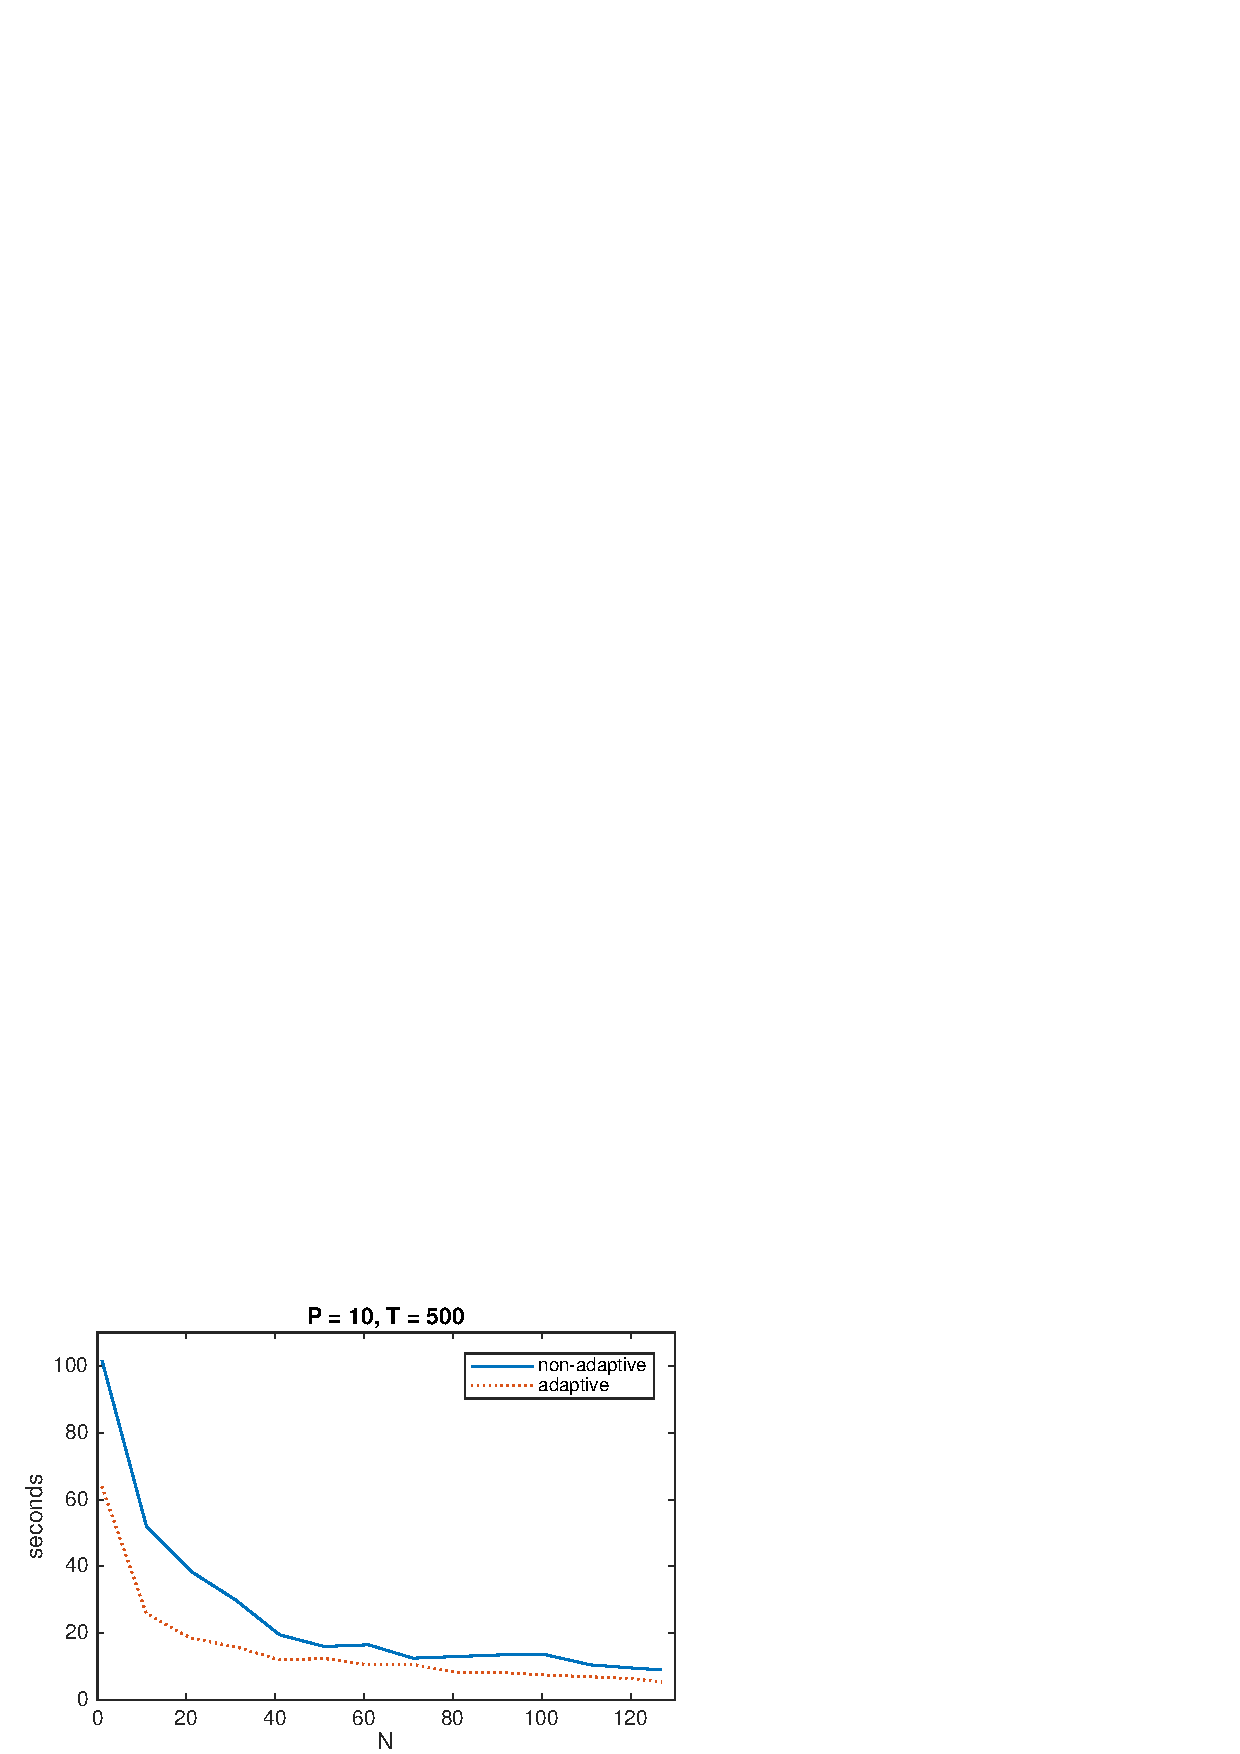
\includegraphics[scale=0.5]{images/N_T500_P10}
	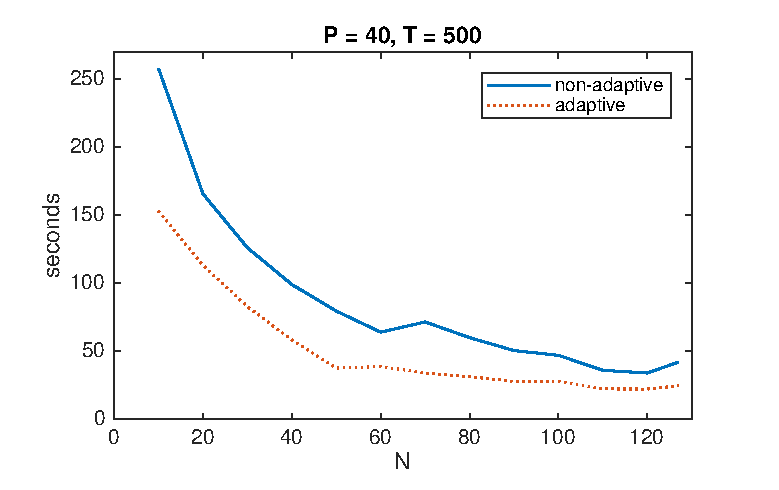
\includegraphics[scale=0.5]{images/N_T500_P40}
	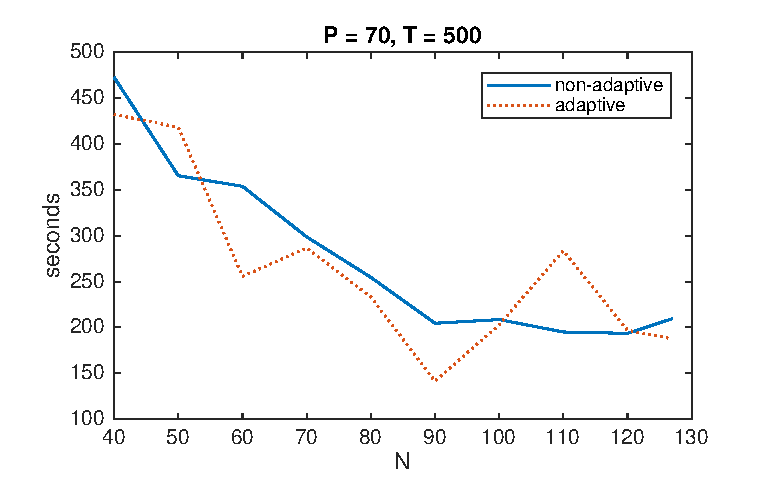
\includegraphics[scale=0.5]{images/N_T500_P70}
	\caption{prestazioni al variare dell'ampiezza della finestra N,
			 timeout T = 500 ms, probabilità di perdita bassa (P = 10\%),
			 media (P = 40\%) e alta (P = 70\%)}
\end{figure}
\begin{figure}[!hp]
	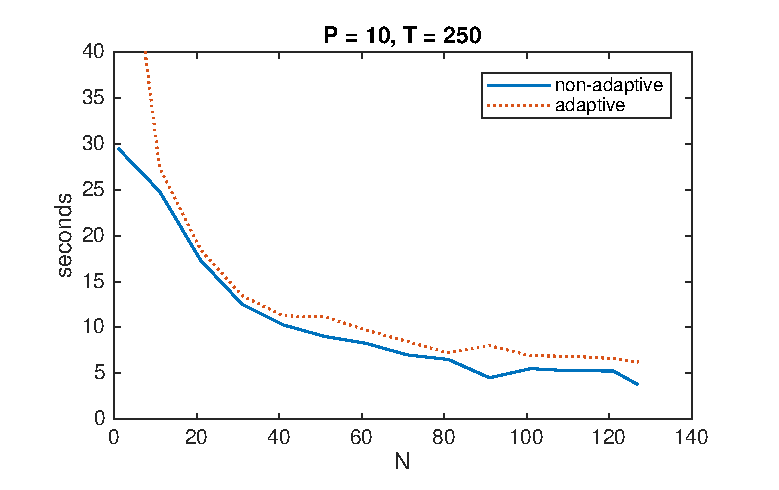
\includegraphics[scale=0.5]{images/N_T250_P10}
	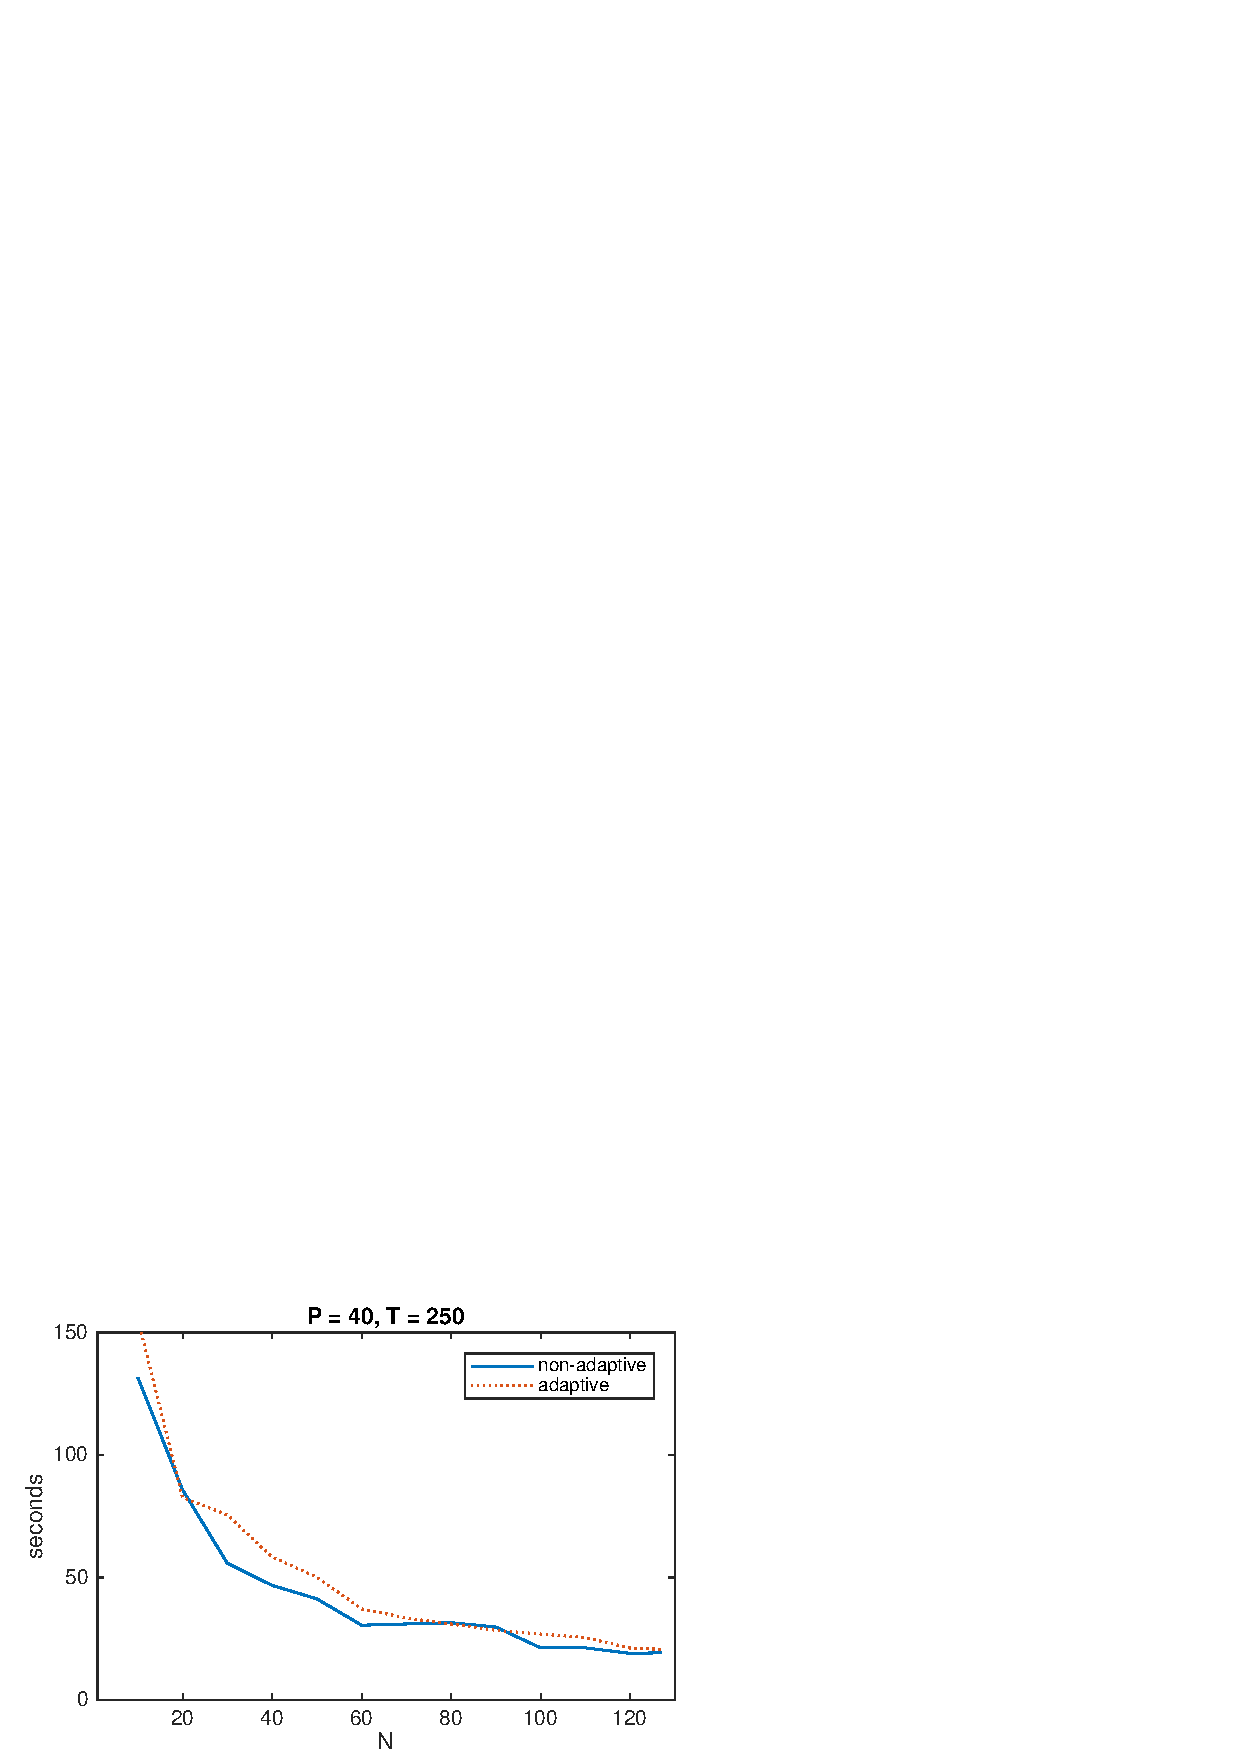
\includegraphics[scale=0.5]{images/N_T250_P40}
	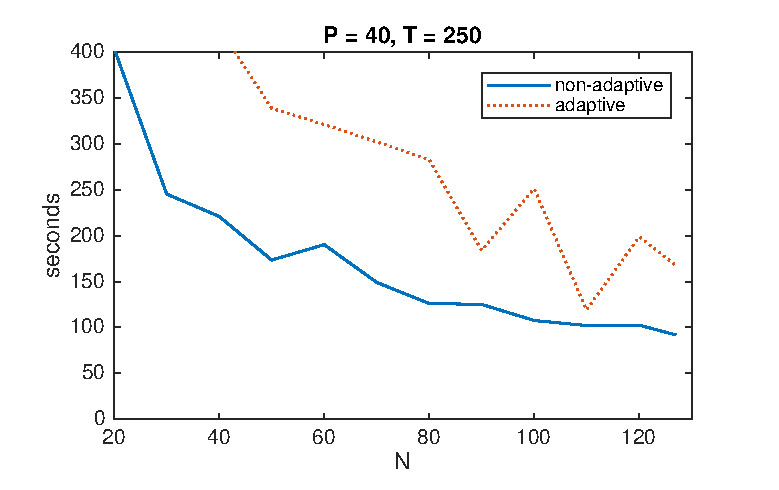
\includegraphics[scale=0.5]{images/N_T250_P70}
	\caption{prestazioni al variare dell'ampiezza della finestra N,
			 timeout T = 250 ms, probabilità di perdita bassa (P = 10\%),
			 media (P = 40\%) e alta (P = 70\%)}
\end{figure}

\subsubsection{Analisi al variare di T}
Per quanto riguarda le prestazioni al variare del valore del timeout,
si osserva (figura \ref{t}) che vi è una crescita lineare del tempo impiegato all'aumentare del
parametro T nel caso di timeout fisso.\\
Nel caso di timeout adattativo, per perdite poco o mediamente frequenti,
il tempo impiegato converge ad un valore costante
proporzionale alla probabilità di perdita,
mentre si conferma molto variabile in caso di elevata probabilità di perdita. 
\begin{figure}[!hp]
	\centering
	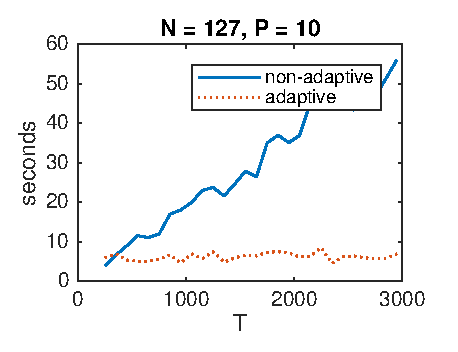
\includegraphics[scale=0.8]{images/T_N127_P10}
	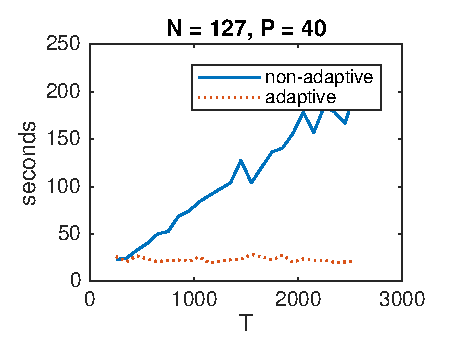
\includegraphics[scale=0.8]{images/T_N127_P40}
	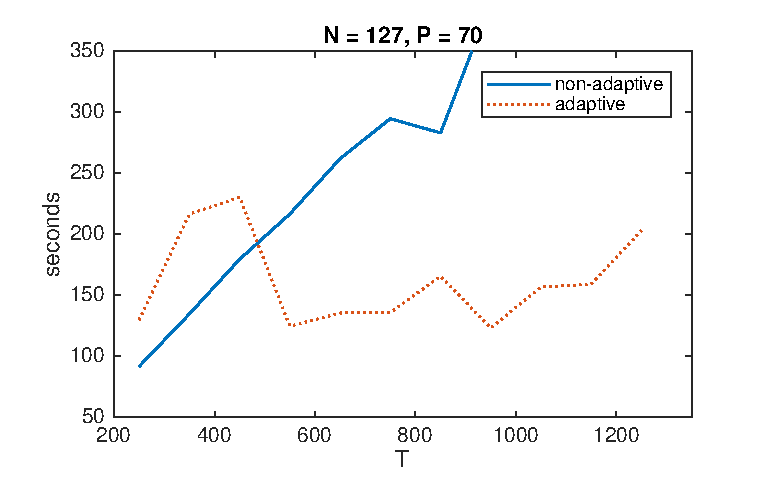
\includegraphics[scale=0.8]{images/T_N127_P70}
	\caption{prestazioni al variare del valore del timeout T,
			 ampiezza finestra N = 127, probabilità di perdita bassa (P = 10\%),
			 media (P = 40\%) e alta (P = 70\%)}
	\label{t}
\end{figure}

\subsubsection {Analisi al variare di P}
Anche al variare della probabilità di perdità si osserva un andamento 
abbastanza lineare fino a valori vicini al 60\%, da questo punto in
poi però, si ha una rapida divergenza e le prestazioni peggiorano
drasticamente.\\
Confermate, anche in questo caso, le peggiori prestazioni della versione
con timeout adattativo rispetto a timeout fisso per probabilità di perdita
elevate.
\begin{figure}[!ht]
	\centering
	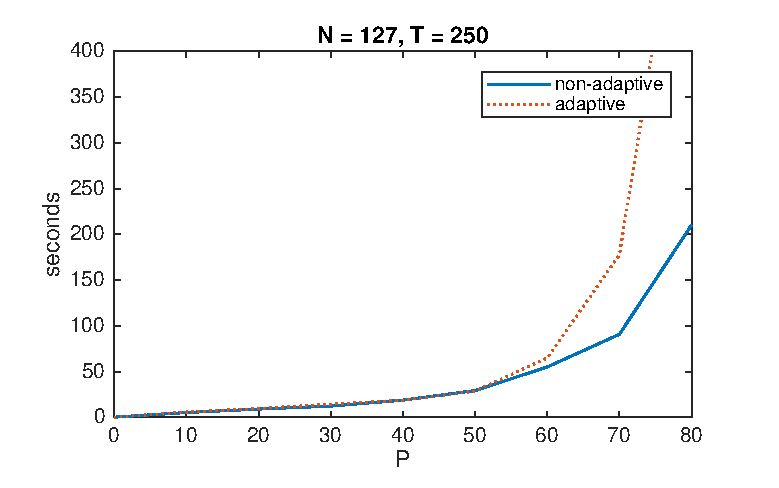
\includegraphics[scale=0.8]{images/P_N127_T250}
	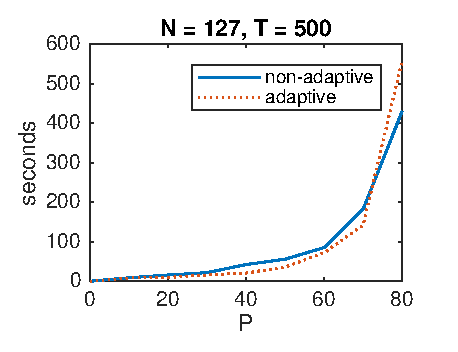
\includegraphics[scale=0.8]{images/P_N127_T500}
	\caption{prestazioni al variare della probabilità di perdita P,
			 ampiezza finestra N = 127, timeout minimo T = 250 ms e 
			 timeout normale T = 500 ms}
\end{figure}
\newpage

%


\section{Installazione e configurazione}
Per avviare l'installazione del sistema basta semplicemente eseguire il file
\emph{install.sh} che farà partire la compilazione del codice sorgente e 
creerà una cartella \emph{server} ed una \emph{client} contenenti i
relativi file binari, inoltre verranno copiati alcuni file di esempio nella
cartella del server per poter testare subito l'applicazione.\\
Se il procedimento non dovesse funzionare provare a concedere i permessi di
esecuzione al file di installazione tramite il comando:

\emph{chmod -x install.sh}\\
oppure provare ad eseguire il file all'interno del terminale:

\emph{./install.sh}


\section{Esempi di funzionamento}
In questo esempio verrà eseguito il sistema su di un'unica macchina
sfruttando l'interfaccia di loopback.
Per eseguire il server aprire il terminale nella cartella \emph{server}
creata durante l'installazione ed eseguire il comando:\\
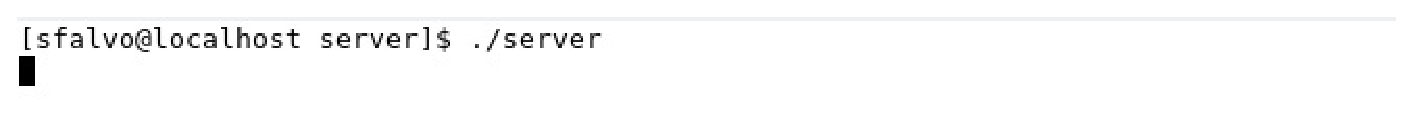
\includegraphics[scale=0.5]{images/esempio/srv_launch}\\
In questo modo viene lanciato il server con i seguenti parametri di default:
\begin{itemize}
\item[T]: 500 
\item[P]: 20
\item[N]: 50
\item[adaptive]: 0 (false)
\item[port]: 5193 
\end{itemize}
Lato client, aprire il terminale nella relativa cartella, ed eseguire il 
comando\\ 
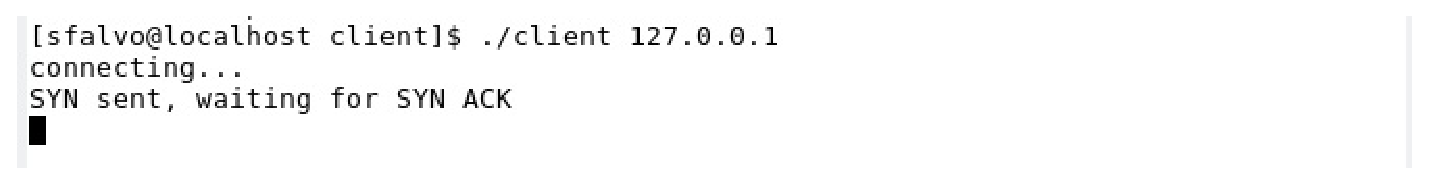
\includegraphics[scale=0.5]{images/esempio/cli_connect}\\
Verra eseguito il client che tenterà ripetutamente di
connettersi al server.\\
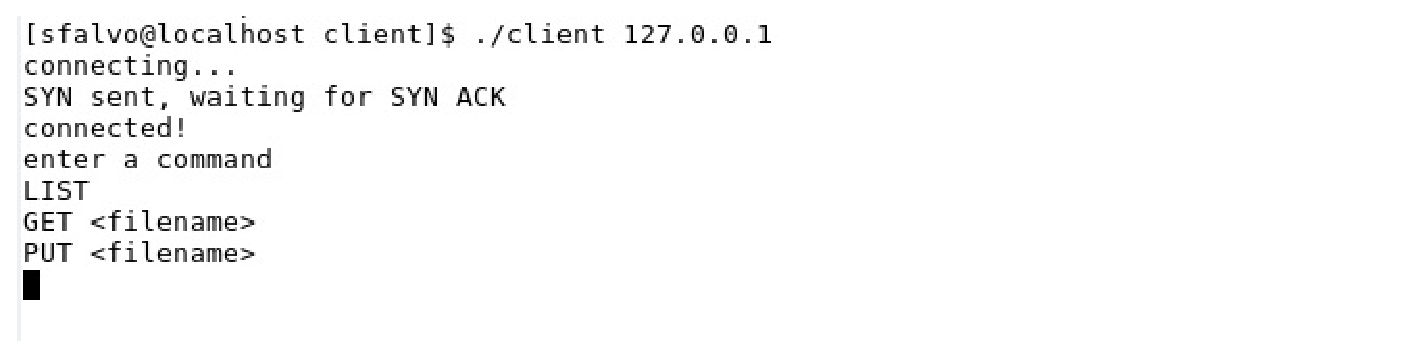
\includegraphics[scale=0.5]{images/esempio/cli_wait}\\
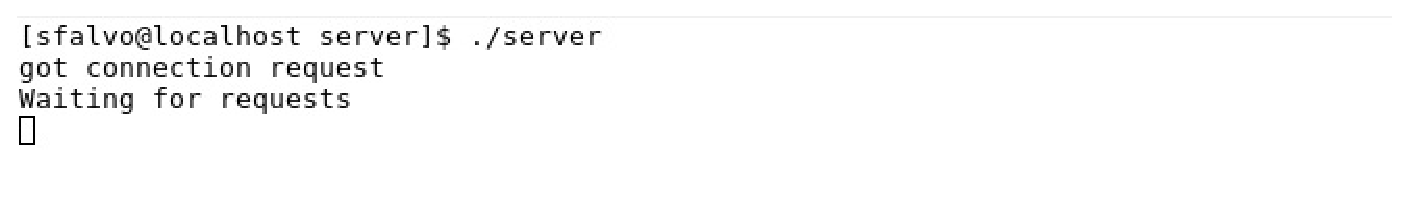
\includegraphics[scale=0.5]{images/esempio/srv_wait}\\
Una volta connessi, inserire uno dei comandi suggeriti, ad esempio il comando LIST\\
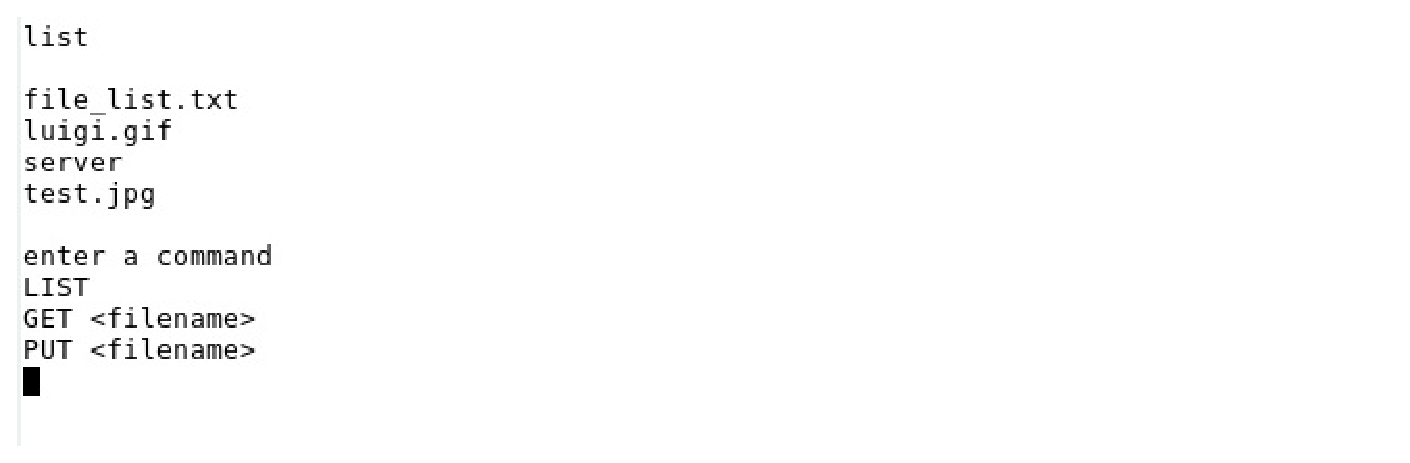
\includegraphics[scale=0.5]{images/esempio/cli_list}\\
Ed ora si può procedere a scaricare uno dei file presenti sul server
tramite il comando GET:\\
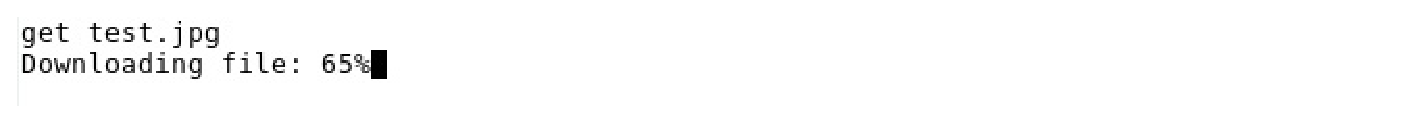
\includegraphics[scale=0.5]{images/esempio/cli_get}\\
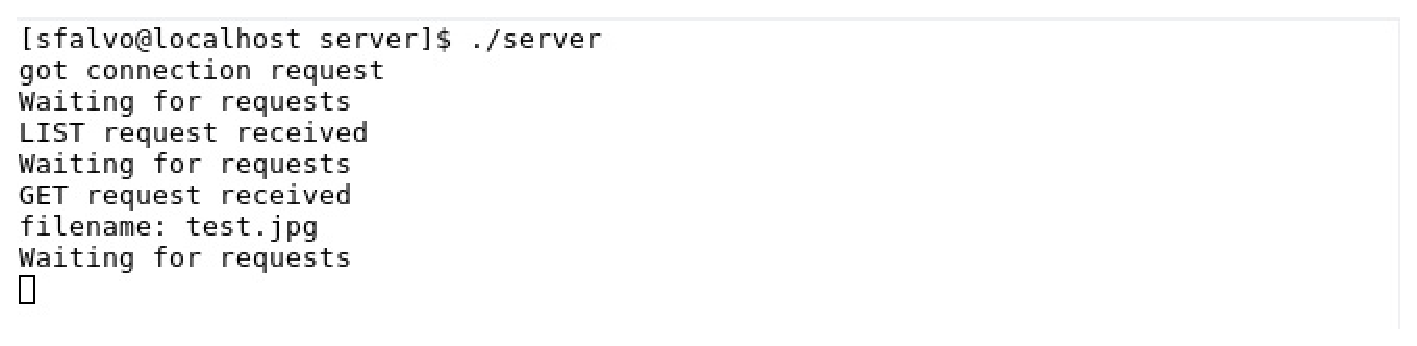
\includegraphics[scale=0.5]{images/esempio/srv_resp}\\
Successivamente si può verificare la presenza del file tramite il comando ls.\\
Per eseguire il server con parametri personalizzati specificare le opzioni
come argomenti del programma, ad esempio:\\
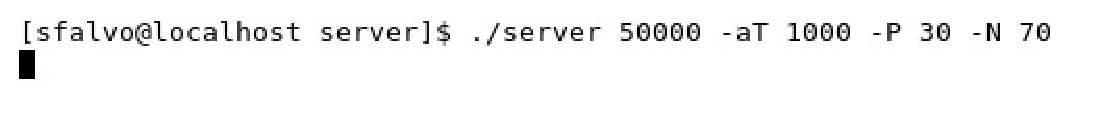
\includegraphics[scale=0.5]{images/esempio/srv_par}\\
In questo modo viene lanciato il server con i seguenti parametri:
\begin{itemize}
\item[T]: 1000
\item[P]: 30
\item[N]: 70
\item[adaptive]: 1 (false)
\item[port]: 5193 
\end{itemize}
Opzioni server:
\begin{itemize}
\item[T]: valore del timeout in millisecondi
\item[P]: probabilità di perdita in percentuale
\item[N]: ampiezza della finestra del protocollo rdt
\item[a]: il protocollo deve avere timeout adattativo
\item[port]: porta di ascolto del server
\end{itemize}
Tutte le opzioni vanno immesse con il trattino che le precede e il valore che le segue.


\begin{thebibliography}{1}
\bibitem{kurose} James F.~Kurose \& Keith W. Ross:
\emph{Reti di calcolatori e internet. Un approccio top-down.}
Pearson (2013)
\end{thebibliography}

\end{document}
